% Auto-generated figure snippets. Every numeric value in the underlying
% plots traces to the experimental log (two-way ANOVA F-statistics and p-values).

% Figure 1: Experimental design schematic
\begin{figure}[htbp]
\centering
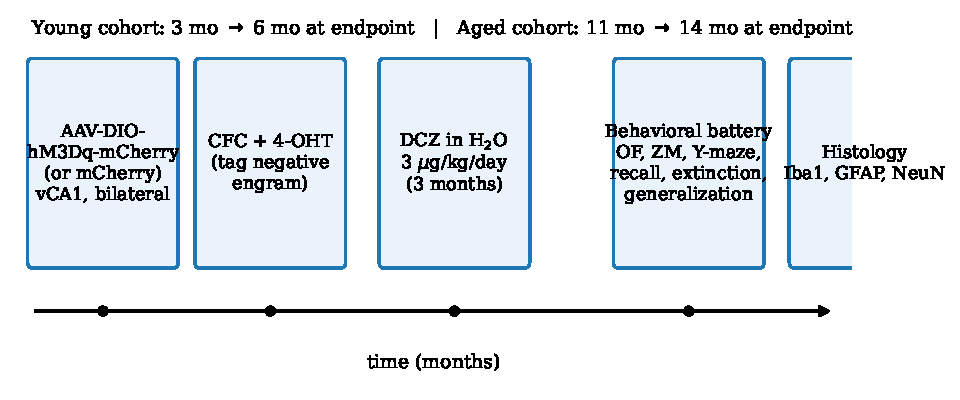
\includegraphics[width=0.95\textwidth]{figures/fig1_design_schematic.pdf}
\caption{\textbf{Experimental design.} TRAP2 mice received bilateral vCA1 injection of AAV9-DIO-Flex-hM3Dq-mCherry or AAV9-DIO-Flex-mCherry (300\,nL total). Two weeks later, contextual fear conditioning (four 1.5\,mA foot shocks in context A) was followed by 40\,mg\,kg$^{-1}$ i.p. 4-OHT to tag the negative engram. Chronic activation used DCZ in home-cage drinking water (3\,$\mu$g\,kg$^{-1}$\,day$^{-1}$, refreshed every 5 days) for 3 months. Young and aged cohorts (3\,mo and 11\,mo at surgery) reached 6\,mo and 14\,mo at endpoint. Endpoint assays: open field (OF), zero maze (ZM), Y-maze, remote recall, extinction, and generalization, followed by histology (Iba1, GFAP, NeuN).}
\label{fig:design}
\end{figure}

% Figure 2: Behavior summary
\begin{figure}[htbp]
\centering
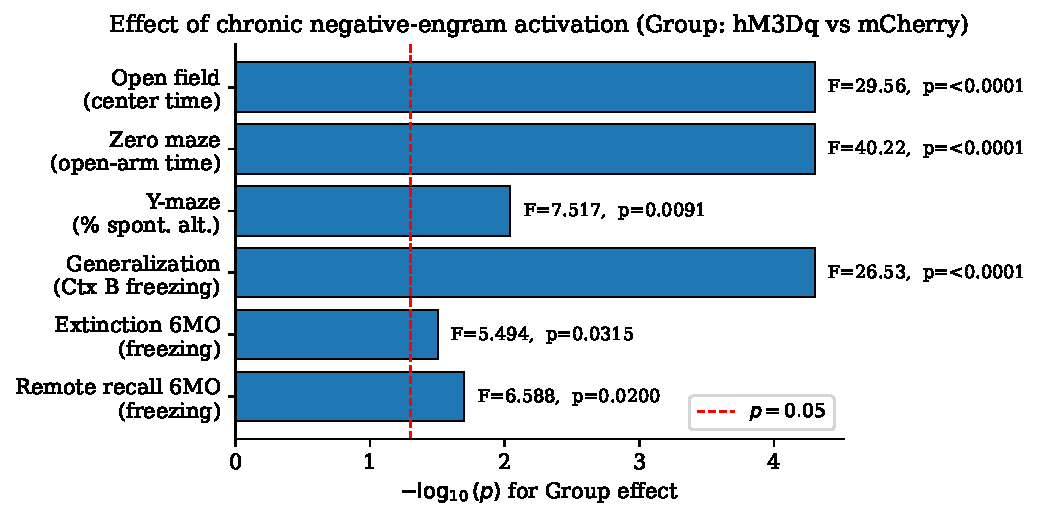
\includegraphics[width=0.85\textwidth]{figures/fig2_behavior_summary.pdf}
\caption{\textbf{Behavioral outcomes across assays, pooled across age.} $-\log_{10}(p)$ of the two-way ANOVA Group main effect (hM3Dq vs mCherry), with the exact $F$ and $p$ values annotated. Significant effects at the Group level are obtained for open-field center time ($F(1,33)=29.56$, $p<0.0001$), zero-maze open-arm time ($F(1,38)=40.22$, $p<0.0001$), Y-maze spontaneous alternation ($F(1,40)=7.517$, $p=0.0091$), Context\,B generalization freezing ($F(1,41)=26.53$, $p<0.0001$), extinction in the 6-month cohort ($F(1,17)=5.494$, $p=0.0315$), and remote recall in the 6-month cohort ($F(1,17)=6.588$, $p=0.0200$).}
\label{fig:behavior}
\end{figure}

% Figure 3: Age-dependence of group effects
\begin{figure}[htbp]
\centering
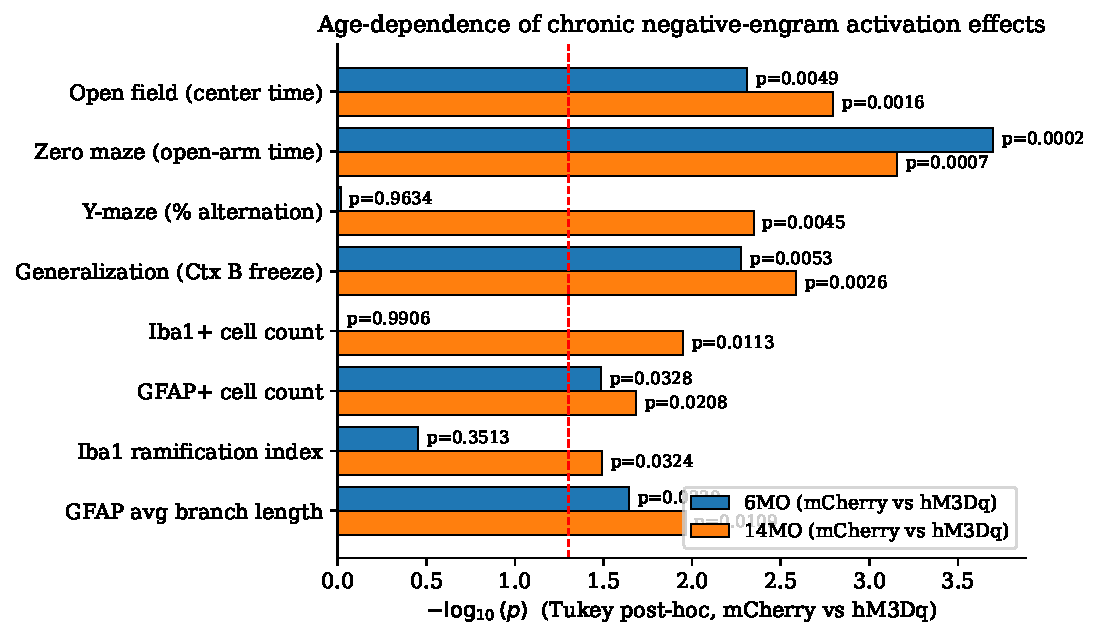
\includegraphics[width=0.9\textwidth]{figures/fig3_age_by_group_tukey.pdf}
\caption{\textbf{Age-by-group Tukey post-hoc comparisons.} Per-age Tukey $p$-values for hM3Dq vs age-matched mCherry, plotted as $-\log_{10}(p)$. Anxiety (open field, zero maze) and context-generalization freezing reach significance at both ages. Y-maze spontaneous alternation is impaired only at 14\,mo (6MO $p=0.9634$; 14MO $p=0.0045$). Iba1+ count increases only at 14\,mo ($p=0.0113$; 6MO $p=0.9906$), whereas GFAP+ count increases at both ages (6MO $p=0.0328$; 14MO $p=0.0208$).}
\label{fig:age_by_group}
\end{figure}

% Figure 4: Glial remodeling summary
\begin{figure}[htbp]
\centering
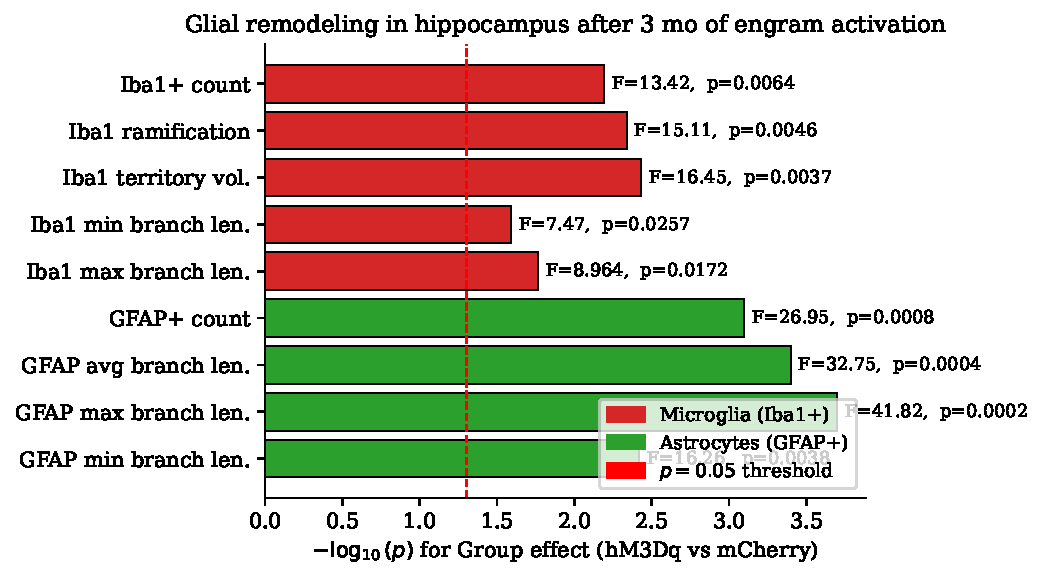
\includegraphics[width=0.85\textwidth]{figures/fig4_glia_summary.pdf}
\caption{\textbf{Glial remodeling in hippocampus after 3 months of chronic negative-engram activation.} Two-way ANOVA Group $F$-statistics and $p$-values for Iba1+ microglia and GFAP+ astrocyte metrics. All measures plotted have a significant Group effect: Iba1+ count ($F(1,8)=13.42$, $p=0.0064$), ramification ($p=0.0046$), territory volume ($p=0.0037$), minimum ($p=0.0257$) and maximum branch length ($p=0.0172$); GFAP+ count ($F(1,8)=26.95$, $p=0.0008$), average ($p=0.0004$) and maximum branch length ($p=0.0002$), and minimum branch length ($p=0.0038$). Age-specific Tukey contrasts are summarized in Fig.~\ref{fig:age_by_group}.}
\label{fig:glia}
\end{figure}

% Figure 5: NeuN safety
\begin{figure}[htbp]
\centering
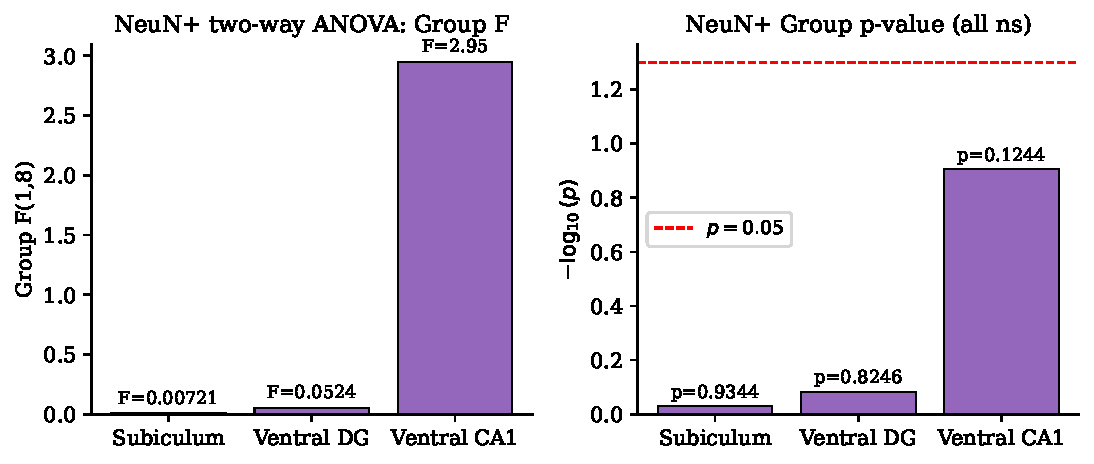
\includegraphics[width=0.85\textwidth]{figures/fig5_neun_safety.pdf}
\caption{\textbf{Chronic activation does not reduce NeuN+ neuron counts.} Two-way ANOVA Group $F$-statistics (left) and $-\log_{10}(p)$ (right) for NeuN+ counts in subiculum (Group $F(1,8)=0.00721$, $p=0.9344$), ventral dentate gyrus ($F(1,8)=0.0524$, $p=0.8246$), and ventral CA1 ($F(1,8)=2.947$, $p=0.1244$). None reach $p=0.05$ (red dashed line).}
\label{fig:neun}
\end{figure}

% Figure 6: Microscopy placeholder
\begin{figure}[htbp]
\centering
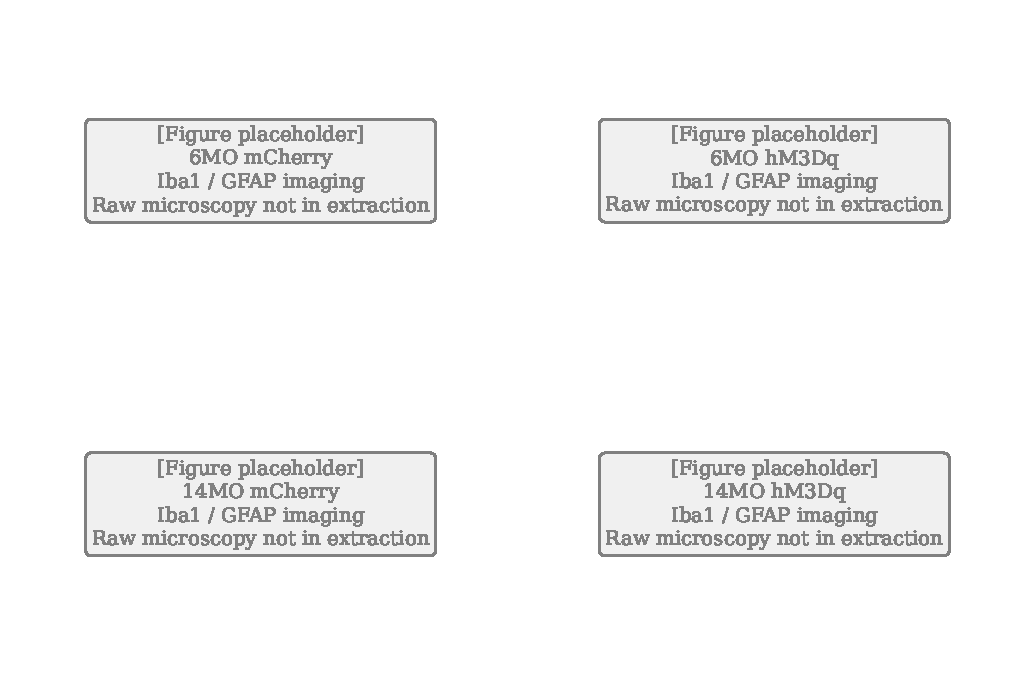
\includegraphics[width=0.8\textwidth]{figures/fig6_microscopy_placeholder.pdf}
\caption{\textbf{Representative Iba1+ and GFAP+ microscopy (placeholder).} Raw imaging panels for 6\,mo and 14\,mo mCherry and hM3Dq mice are shown schematically; the corresponding 3DMorph-derived quantifications are plotted in Figs.~\ref{fig:glia} and \ref{fig:age_by_group}.}
\label{fig:microscopy}
\end{figure}
